\paragraph{エージェント}
エージェントはドローン本体とし、以下の様な仕様とした。
\begin{itemize}
    \item 飛行航路検索はUnityの一機能であるナビゲーションメッシュを使用したパス検索を応用
    \item 観測(モデルへの入力)
    \begin{itemize}
        \item 自身の位置/速度/モード/目的地/誘導人数
        \item 他エージェントの 位置/誘導人数/モード/目的地
        \item 各タワーの現在の避難可能人数
        \item レイキャストで観測した避難者の位置
    \end{itemize}
    \item 行動(モデルの出力)
    \begin{itemize}
        \item 探索時:ナビメッシュ上で任意の地点を目的地に指定
        \item 誘導時:タワーを目的地に指定
    \end{itemize}
    \item 報酬
    \begin{itemize}
        \item エピソード終了時タワーまで誘導できた人数を報酬
        \item (個別報酬)0人の場合は、報酬 -1
        \item (全体報酬):エージェント報酬の合計
    \end{itemize}
\end{itemize}
\begin{figure}[H]
    \centering
    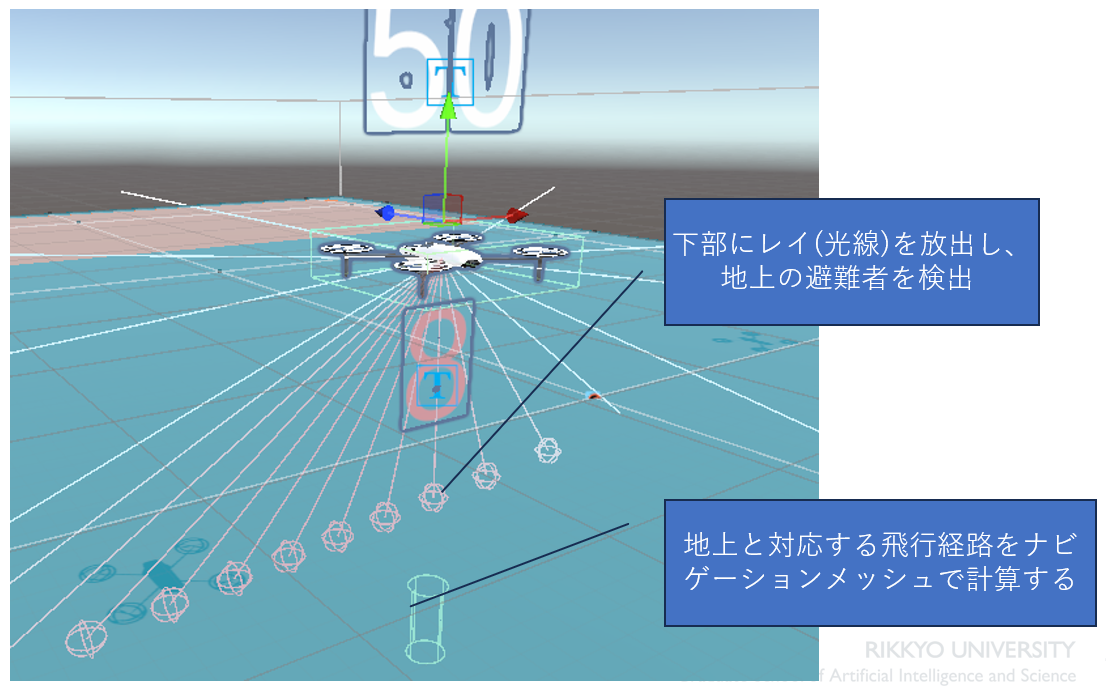
\includegraphics[scale=0.5]{./images/droneagent.png}
    \caption{
       ドローンエージェント
    }
\end{figure}
    
\paragraph{避難者}
避難者のアルゴリズムとしては以下の様な仕様とした。
\begin{figure}[H]
    \centering
    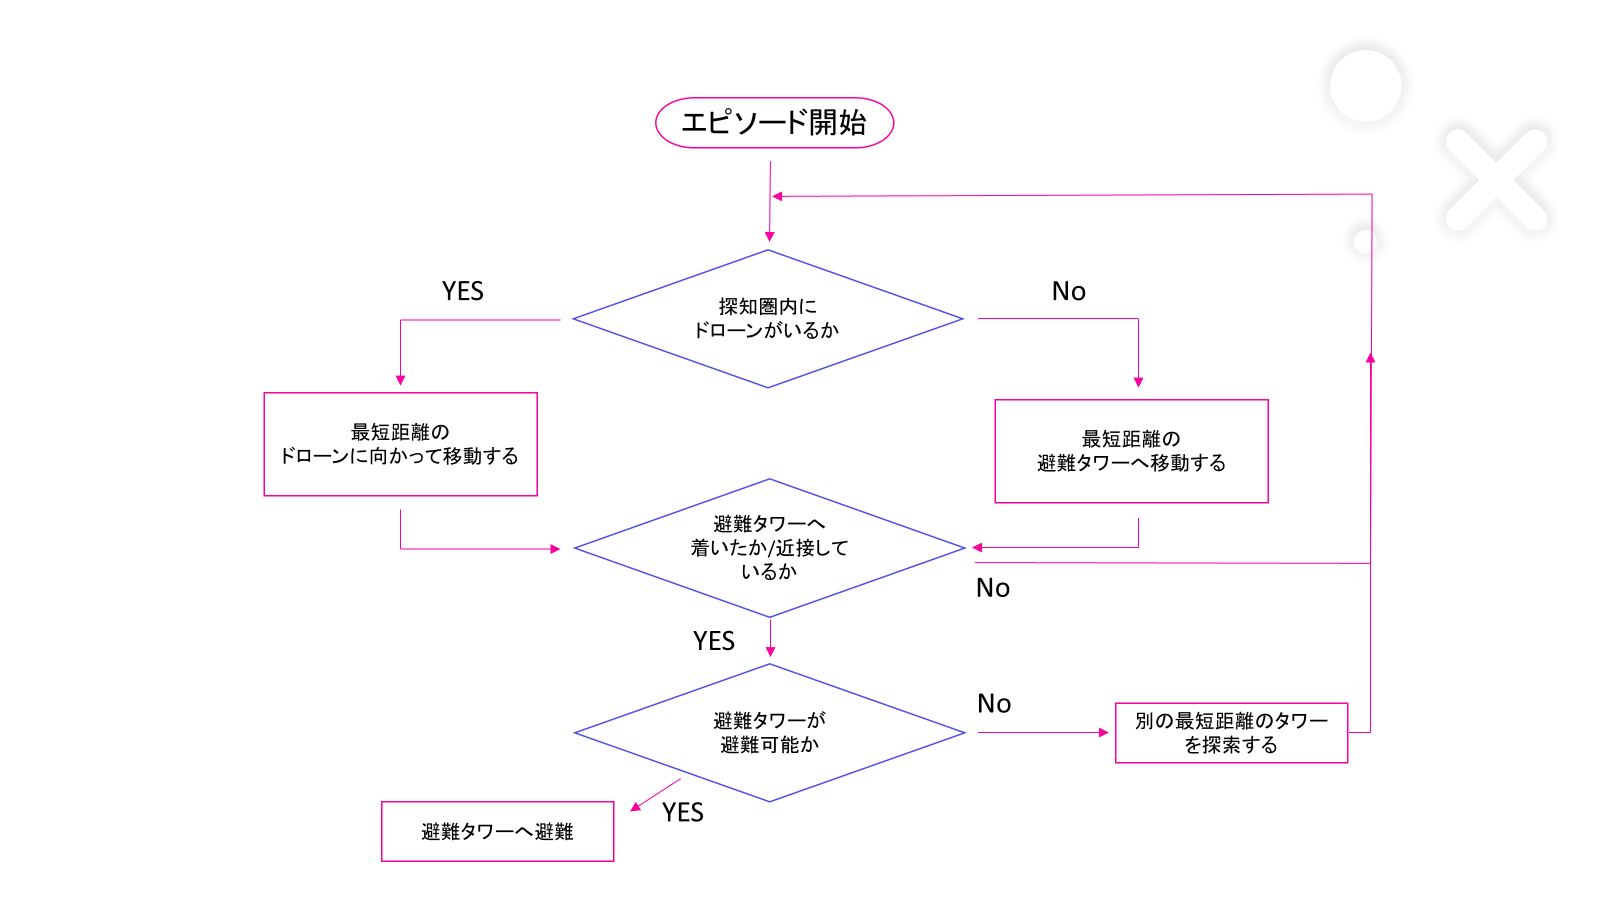
\includegraphics[scale=0.8]{./images/334170449-c22ed682-06c1-4fbc-ba4b-07d946d8a047.png}
    \caption{
       避難者の行動フローチャート
    }
\end{figure}